\begin{block}{\large \smash{Future use}\vphantom{Future}}
\begin{columns}[T]
\begin{column}{0.01\linewidth}\end{column}
\begin{column}{0.313\linewidth}
\begin{itemize}
    \item Embedded System Toolchain Development
    \item Code Testing \& Debugging
    \item Hardware Prototyping
    \item Model Checking
\end{itemize}
\end{column}
\begin{column}{0.01\linewidth}\end{column}
\begin{column}{0.313\linewidth}
  \begin{figure}[!htb]
    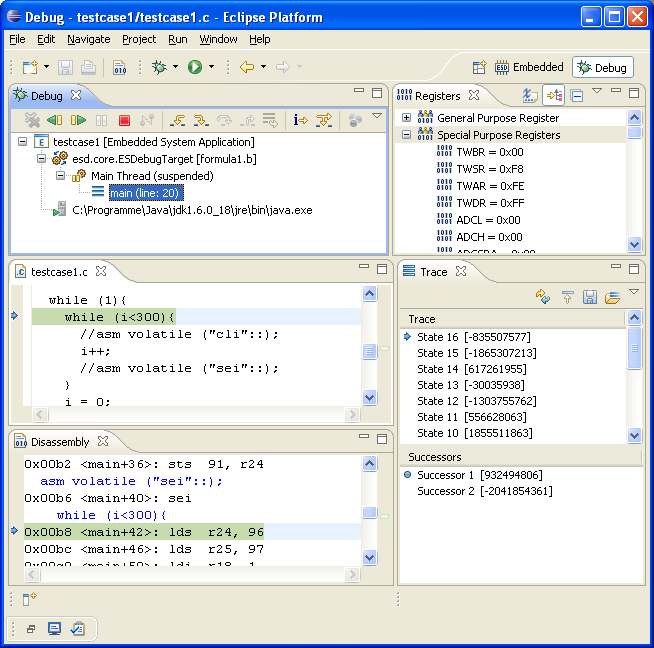
\includegraphics{figures/overview.jpg}
    \caption{Embedded System Toolchain Development}
  \end{figure}
\end{column}
\begin{column}{0.313\linewidth}
\begin{figure}[h!]
\subfigure[Model checking]{
\begin{tikzpicture}[scale=0.7, transform shape]
\node[] (sinit) {};
\node[cloud, fill=white, draw=black, cloud puffs=15, aspect=2.5, inner sep=0pt, cloud puff arc=120, text=black] (s0) [right of=sinit, node distance=7cm] {\bf $\mathrlap{\text{\ \ \ \ System}}$\phantom{Requirements}};
\node[smallrectangle] (s1) [below of=s0, node distance=7cm] {$\mathrlap{\text{\ \:Model}}\phantom{Property}$};
\node[cloud, fill=white, draw=black, cloud puffs=15, aspect=2.5, inner sep=0pt, cloud puff arc=120, text=black] (s2) [right of=s0, node distance=15cm] {\bf Requirements};
\node[smallrectangle] (s3) [below of=s2, node distance=7cm] {Property};
\draw[->] (s0) edge (s1);
\draw[->] (s2) edge (s3);
\node[] (temp) [below of=s1, node distance=6cm] {};
\node[smallrectangle] (s4) [right of=temp, node distance=7.5cm] {Model checker};
\draw[->] (s1) edge (s4);
\draw[->] (s3) edge (s4);
\node[oval, inner sep=0.4cm, fill=red] (s5) [left of=s4, node distance=9cm] {Fail};
\node[oval, inner sep=0.4cm, fill=green] (s6) [right of=s4, node distance=9cm] {Pass};
\draw[->] (s4) edge (s5);
\draw[->] (s4) edge (s6);
\draw[->] (s5) edge (s1);

\end{tikzpicture}
}
\end{figure}
\end{column}
\begin{column}{0.01\linewidth}\end{column}
\end{columns}
\end{block}
